\chapter{Acoustic waves and waveguides}

In this chapter, the theory of the physics behind my simulations is given.
\Cref{sec:acoustics} gives a review of solid mechanics in the frequency domain,
culminating in \cref{eq:gov_eq}, which is the equation that is solved each
simulation.
\Cref{sec:bloch} goes on to show that the solutions to this equation with no
external forces for infinite periodic structures can be obtained from simulating
a single unit cell of the structure.
Lastly, the solutions for the specific periodic structure used for the inputs
and outputs in this thesis is shown with a band diagram as well as the shapes of
the modes.

\section{The frequency domain acoustic equation}\label{sec:acoustics}

In order to efficiently model the deformation and stresses in a solid material,
a linear elasticity model is often assumed.
For small deformations, solid materials obey Hooke's law which in it's full form
looks like
\begin{equation}\label{eq:stress}
	\sigma = C : \epsilon
\end{equation}
where $\sigma$ is the stress tensor, $C$ the elasticity tensor which is a
rank four tensor that is a property of the material,
\begin{equation}\label{eq:strain}
	\epsilon \coloneqq \frac12(\nabla \vec u + (\nabla \vec u)^\transpose)
\end{equation}
is the strain tensor, and $:$ denotes double scalar product%
\footnote{%
	See \cref{eq:double_scalar_product_index_not} for what the double scalar
	product means in this case. It is in general a product that contracts two
	indices, as opposed to the regular scalar product that contracts only one.
}%
.
This equation is linear in $\vec u$, hence the name \emph{linear} elasticity.
Using this and Newton's equations of motion, the equation governing the dynamics
is obtained:
\begin{equation}\label{eq:lin_el}
	\rho \ddot{\vec{u}} = \nabla \cdot \sigma + \vec F,
\end{equation}
where $\rho$ is the density, $\vec{u}$ is the displacement and $\vec F$ is the
externally applied force.
Assuming a time harmonic solution
$\vec u(\vec x, t) = \vec u(x) e^{i \omega t}$
with angular frequency $\omega$ this becomes
\begin{equation}\label{eq:lin_el2}
	-\rho \omega^2 \vec{u} = \nabla \cdot \sigma + \vec F.
\end{equation}

To combine \cref{eq:stress,eq:strain,eq:lin_el,eq:lin_el2} into one equation that can be solved for $\vec{u}$ we first
rewrite them in index notation to make calculations clearer:
\begin{align}
	\epsilon_{ij} &= \frac12(\partial_i u_j + \partial_j u_i)\\
	\label{eq:double_scalar_product_index_not}
	\sigma_{ij} &= C_{ijkl} \epsilon_{kl}\\
				&= \frac12\left(C_{ijkl} \partial_k u_l + C_{ijkl} \partial_l
				u_k\right)\\
				&= C_{ijkl} \partial_k u_l\text{ because of the symmetry
				$C_{ijkl}=C_{ijlk}$}
\end{align}
which gives
\begin{align}
	F_{i} &= -\rho \omega^2 u_{i} - \partial_j \sigma_{ij}\\
		   &= -\rho \omega^2 \delta_{ik} u_{k} -
		   \partial_j \left(C_{ijkl} \partial_l u_k\right)\\
		   &= -\left(\rho \omega^2 \delta_{ik} \placeholder + 
		   \partial_j \left(C_{ijkl} \partial_l \placeholder\right)\right) u_k
\end{align}
where the indices $i,j,k,l$ go over the spatial dimensions $x,y,z$.
Note that throughout this thesis, the Einstein summation convention is used,
meaning that repeated indices are summed.
All of the tensors in the equation above are really tensor fields, i.e.\ they are
functions of $\vec{x}$.
Defining the operator
\begin{equation}\label{eq:A_def}
	\hat A_{ik} =
	-\left(\rho \omega^2 \delta_{ik} \placeholder +
	\partial_j \left(C_{ijkl} \partial_l \placeholder\right)\right)
\end{equation}
we can write
\begin{equation}\label{eq:gov_eq}
	\hat A_{ik} u_k = F_i
\end{equation}

\section{Bloch States and Band Diagrams}\label{sec:bloch}

With no external forces, i.e.\ $F_i = 0$, \cref{eq:gov_eq} can be written as
\begin{equation}
	\frac 1 \rho \partial_j \left(C_{ijkl} \partial_l u_k\right) = \omega^2 u_i,
\end{equation}
which is an eigenvalue equation for the operator
$\hat O_{ik} = \frac 1 \rho\partial_j \left(C_{ijkl} \partial_l \placeholder\right)$
where eigenvalues are the angular frequency squared.
If furthermore the structure is periodic, then the eigenstates are so called
\emph{Bloch states}.

If the structure is periodic in the $y$ direction with some periodicity
$\vec a = a \hat{\vec y}$,
meaning that $C_{ijkl}(\vec x) = C_{ijkl}(\vec x + n \vec a)$ and $\rho(\vec x)
= \rho(\vec x + n \vec a)$ where $n$ is an
integer, then this operator commutes with the translation operator
$\hat T_{\vec a}[\vec u(\vec x)] = \vec u(\vec x + \vec a)$.
This means that there is a basis of simultaneous eigenstates of both operators.
The eigenfunctions of the translation operator are
$\vec f(x, z)\exp(i k_y y)$, where $\vec f$ is an arbitrary function,
and the eigenvalues are $\exp(i k_y a)$.
Defining the reciprocal lattice constant $b = 2 \pi / a$, we see
that the functions $\vec f(x, z) \exp(i (k_y + m b) y)$ for integer values
of $m$ all have the same eigenvalue, which means that they form a degenerate
subspace of eigenfunctions.
This also means that we can restrict ourselves to the first Brillouin zone:
$k_y \in [-b/2, b/2]$,
since any $k_y$ outside this interval can be written as $k_y' + mb$ with
$k_y' \in [-b/2, b/2]$.
Thus, the simultaneous eigenstate $\vec u_{k_y, \omega^2}$ can be written
\begin{equation}
	\vec u_{k_y, \omega^2}(\vec x) = \sum_m \vec f_{m,k_y,\omega^2}(x, z) e^{i (k_y + m b) y}
	= e^{i k_y y} \tilde{\vec f}_{k_y, \omega^2}(\vec x)
\end{equation}
where $\tilde{\vec f}_{k_y, \omega^2}$ is a periodic function with periodicity
$\vec a$ by construction~\cite{joannopoulos2008photonic}.

The solutions to these eigenvalue equations are often called modes, and each
mode has both a frequency and a wave vector. This gives rise to a band diagram,
where the frequency is plotted as a function of the wave vector.

\subsection{Concrete example of phononic crystal}

In this work, a rectangular silicon waveguide patterned with elliptic holes is used.
The structure is clamped at the bottom (meaning that we use a fixed boundary
condition there, enforcing $\vec u = 0$) while the other sides are free.
A top down schematic of the unit cell can be seen in \cref{fig:unitcell}.
The reason for using this specific unit cell is that it has been shown to
enable good coupling between optical and mechanical modes while still being
clamped to a substrate, which improves thermal
properties~\cite{kolvik_clamped_2023}.

\begin{figure}[htpb]
\begin{center}
	\begin{tikzpicture}[scale=6]
	\def \a{0.5}
	\def \w{1.0}
	\def \hx{0.13}
	\def \hy{0.3}
	\def \fadedist{0.15}

	\draw[ultra thick] (-0.5*\w, -0.5*\a) rectangle (0.5*\w, 0.5*\a);
	\draw[ultra thick] (0, 0) circle [x radius=\hy, y radius=\hx];
	\draw[ultra thick, path fading=south]
		(-0.5*\w, -0.5*\a-\fadedist) --
		(-0.5*\w, -0.5*\a)
		(+0.5*\w, -0.5*\a) --
		(+0.5*\w, -0.5*\a-\fadedist);
	\draw[ultra thick, path fading=north]
		(-0.5*\w, 0.5*\a+\fadedist) --
		(-0.5*\w, 0.5*\a)
		(+0.5*\w, 0.5*\a) --
		(+0.5*\w, 0.5*\a+\fadedist);
	\draw[<->]
		(0.4*\w, -0.5*\a*0.95) -- node[right] {$a$}
		(0.4*\w, 0.5*\a*0.95);
	\draw[<->]
		(-0.5*\w*0.95, 0.6*\a) -- node[above] {$w$}
		(0.5*\w*0.95, 0.6*\a);
	\draw[<->] (0,0) -- node[right] {$h_y$} (0.0, 0.95*\hx);
	\draw[<->] (0,0) -- node[below] {$h_x$} (0.95*\hy, 0);
\end{tikzpicture}
\end{center}
\caption{Top down view of unit cell of a phononic crystal.}%
\label{fig:unitcell}
\end{figure}

An infinite waveguide can be simulated with just one unit cell using periodic
boundary conditions at the edge where the unit cell would be attached to the
next one.
As \cref{sec:bloch} showed,
waves with any $\vec k$ can be investigated with a single unit cell since $\vec
u$ is a phase factor $e^{i\vec k \cdot \vec x}$ times some function with the
same periodicity as the unit cell.
Enforcing a wave vector $\vec k = k\hat{\vec y}$
thus entails using periodic boundary conditions with a specified phase shift
over the unit cell.
These are called \emph{floquet periodic boundary conditions} in COMSOL, which is
the simulation software used throughout this thesis.
Running simulations with different $k$
to find the eigenmodes with their
corresponding frequencies for this structure yields the band diagram in
\cref{fig:banddiagram}.
The parameter values used in the simulations can be found in \cref{tab:params}.
\Cref{fig:modeshapes} shows the shapes of the eight lowest lying eigenmodes at
$k=0.9 \pi / a$.
\begin{figure}[htpb]
	\centering
	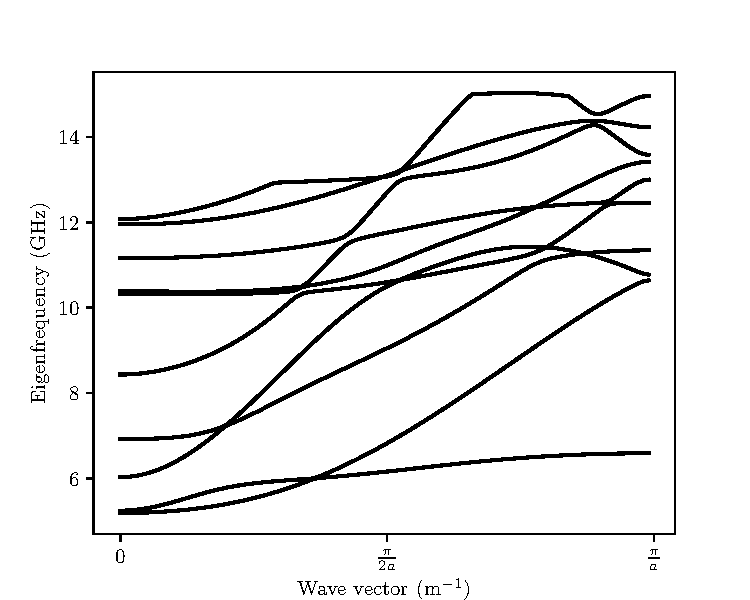
\includegraphics{chapters/theory/bandstructure.pdf}
	\caption{%
		Band diagram of phononic crystal defined in \cref{fig:unitcell}.
	}%
	\label{fig:banddiagram}
\end{figure}

\begin{figure}[htpb]
	\centering
	\begin{subfigure}[]{0.24\textwidth}
		\begin{center}
			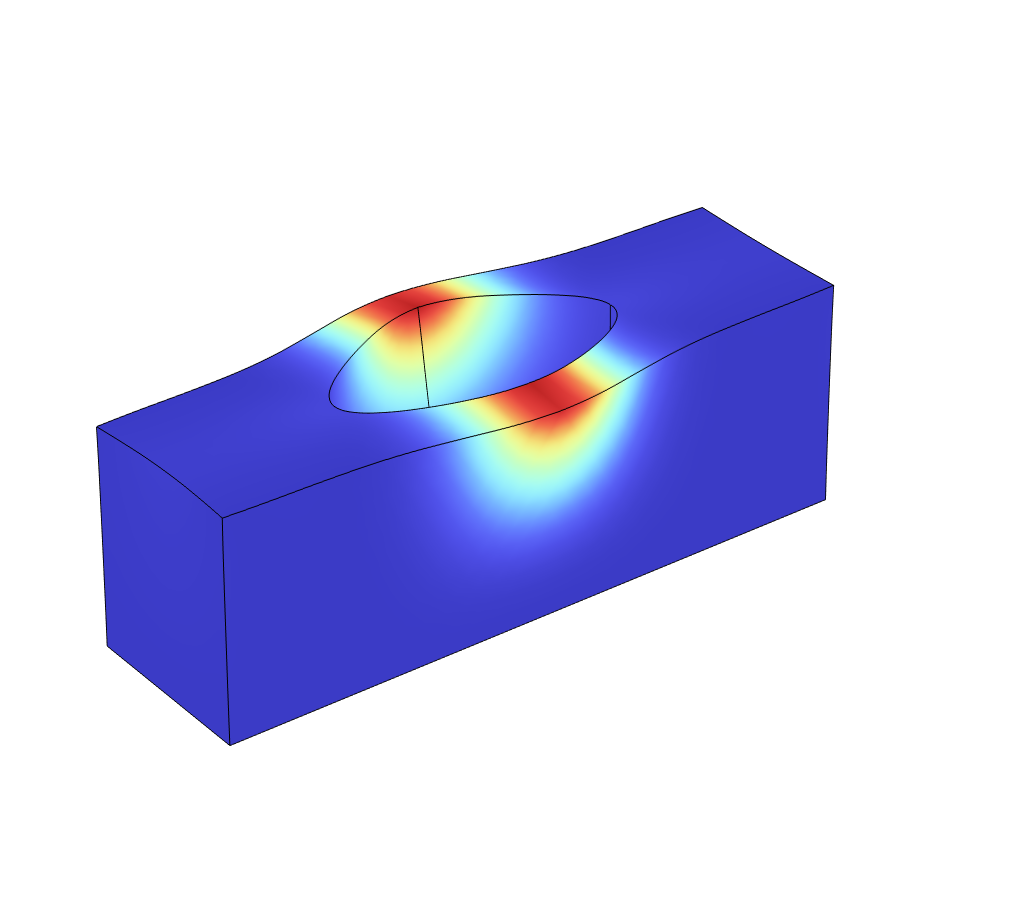
\includegraphics[width=\textwidth]{chapters/theory/modeshape_1.png}
		\end{center}
		\subcaption{}%
		\label{fig:ms1}
	\end{subfigure}
	\begin{subfigure}[]{0.24\textwidth}
		\begin{center}
			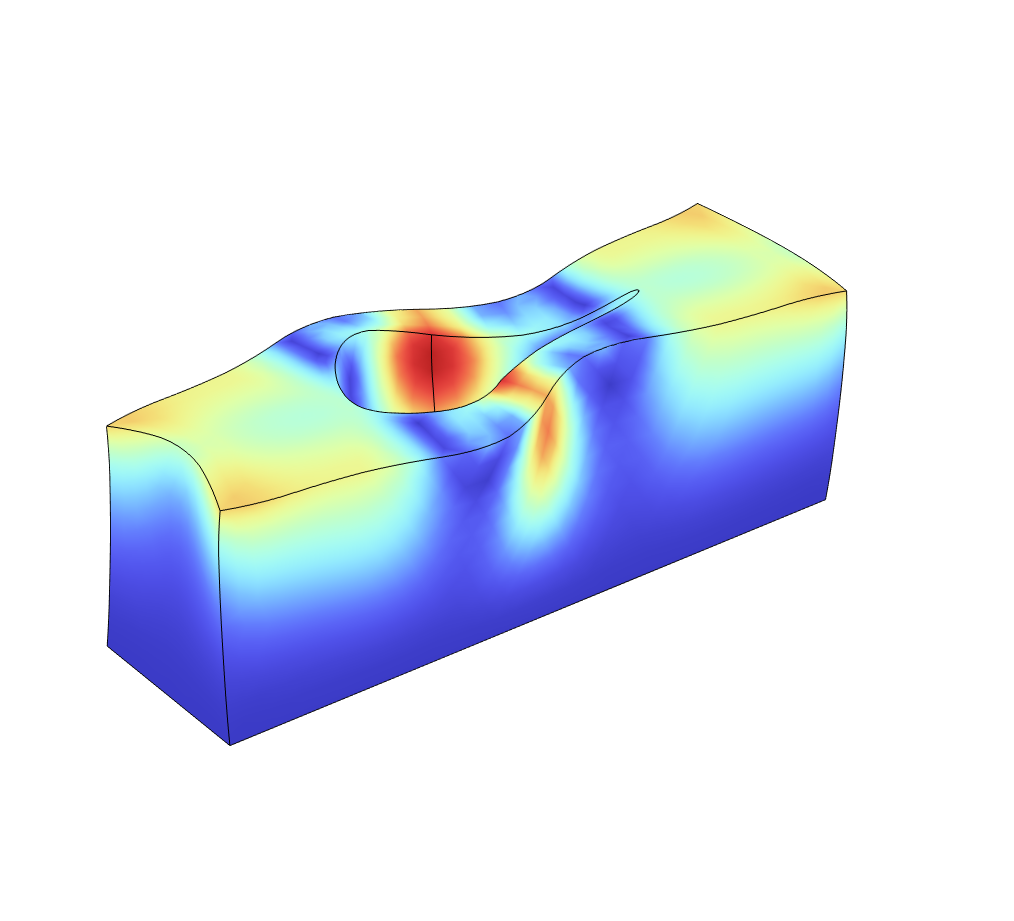
\includegraphics[width=\textwidth]{chapters/theory/modeshape_2.png}
		\end{center}
		\subcaption{}%
		\label{fig:ms2}
	\end{subfigure}
	\begin{subfigure}[]{0.24\textwidth}
		\begin{center}
			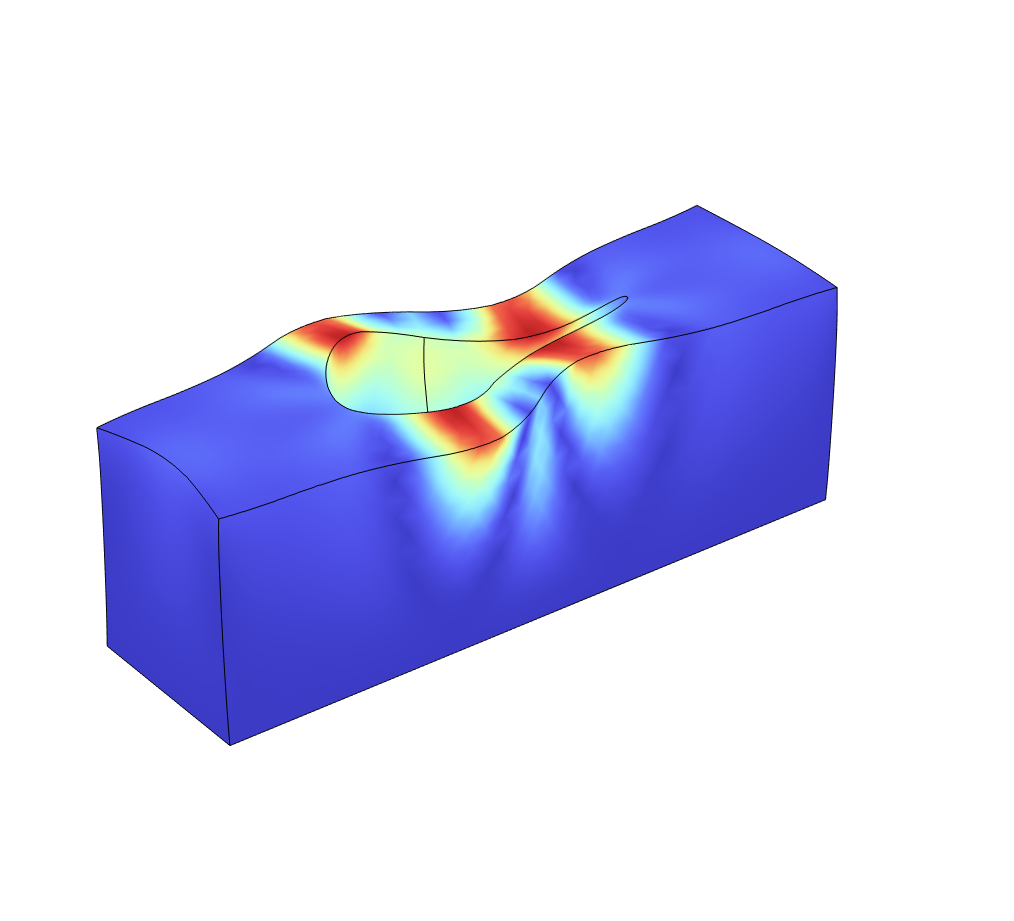
\includegraphics[width=\textwidth]{chapters/theory/modeshape_3.png}
		\end{center}
		\subcaption{}%
		\label{fig:ms3}
	\end{subfigure}
	\begin{subfigure}[]{0.24\textwidth}
		\begin{center}
			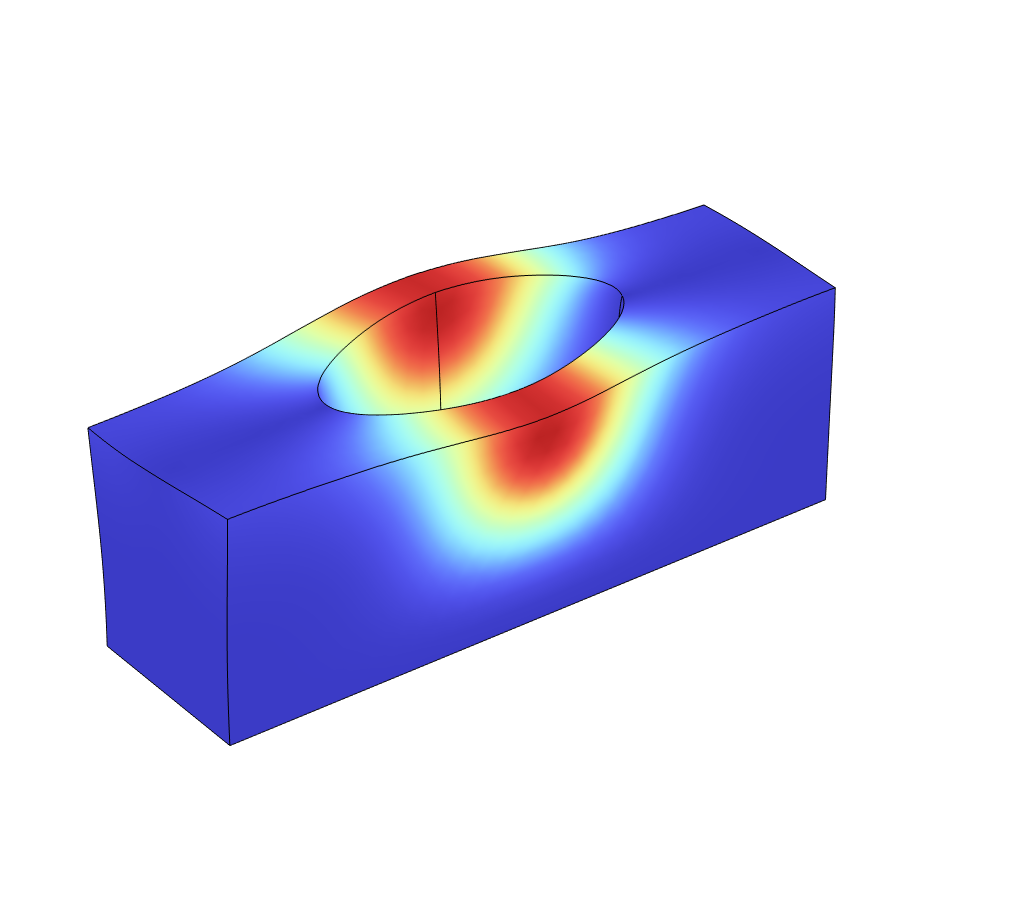
\includegraphics[width=\textwidth]{chapters/theory/modeshape_4.png}
		\end{center}
		\subcaption{}%
		\label{fig:ms4}
	\end{subfigure}\\

	\begin{subfigure}[]{0.24\textwidth}
		\begin{center}
			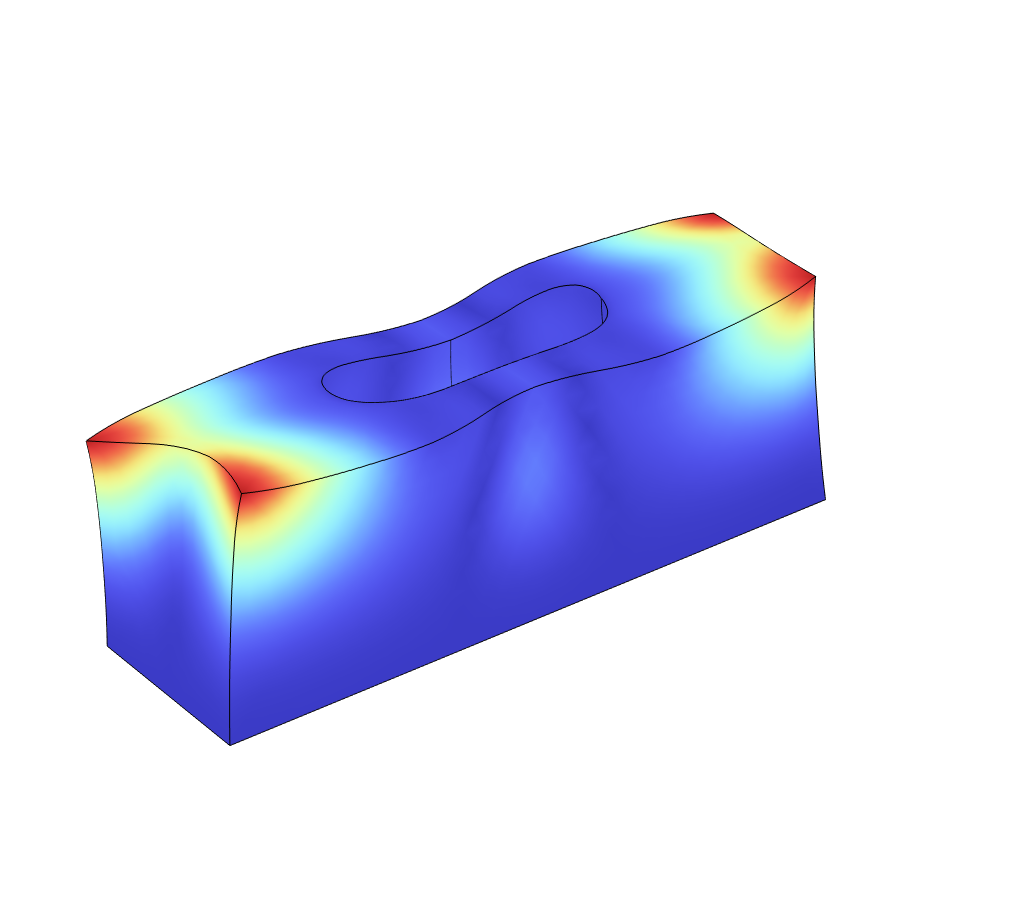
\includegraphics[width=\textwidth]{chapters/theory/modeshape_5.png}
		\end{center}
		\subcaption{}%
		\label{fig:ms5}
	\end{subfigure}
	\begin{subfigure}[]{0.24\textwidth}
		\begin{center}
			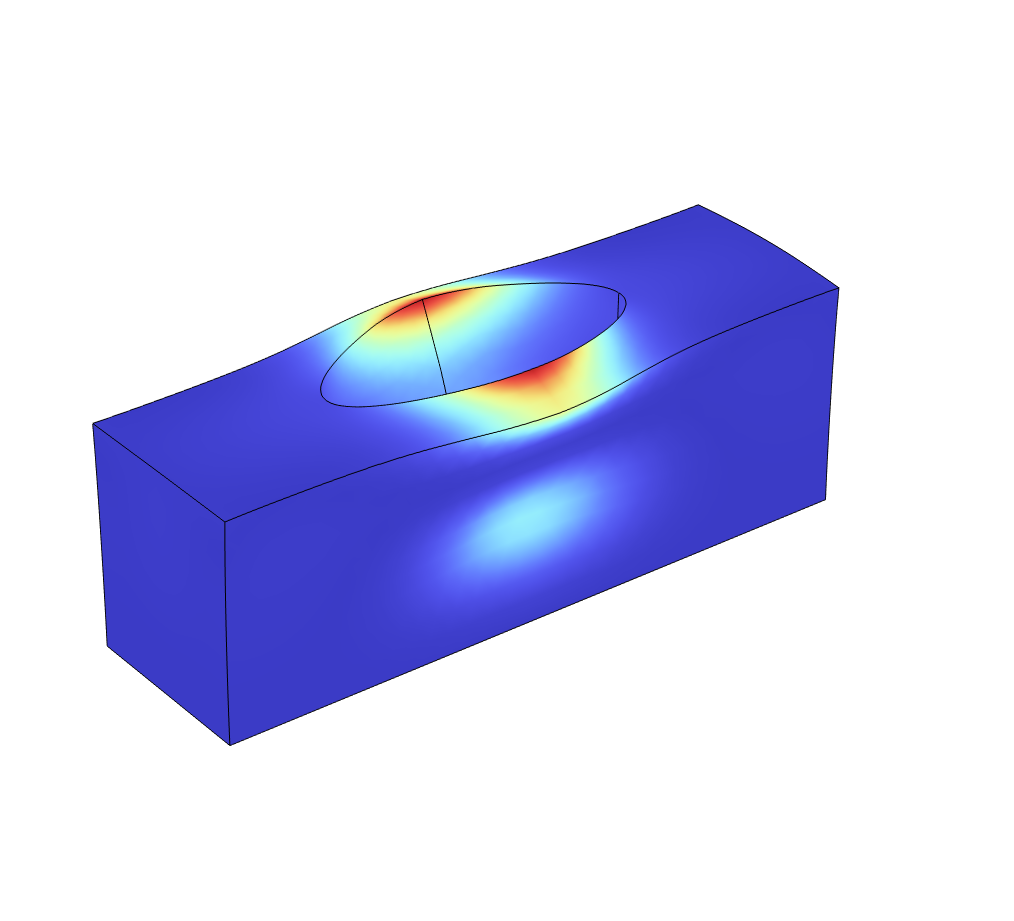
\includegraphics[width=\textwidth]{chapters/theory/modeshape_6.png}
		\end{center}
		\subcaption{}%
		\label{fig:ms6}
	\end{subfigure}
	\begin{subfigure}[]{0.24\textwidth}
		\begin{center}
			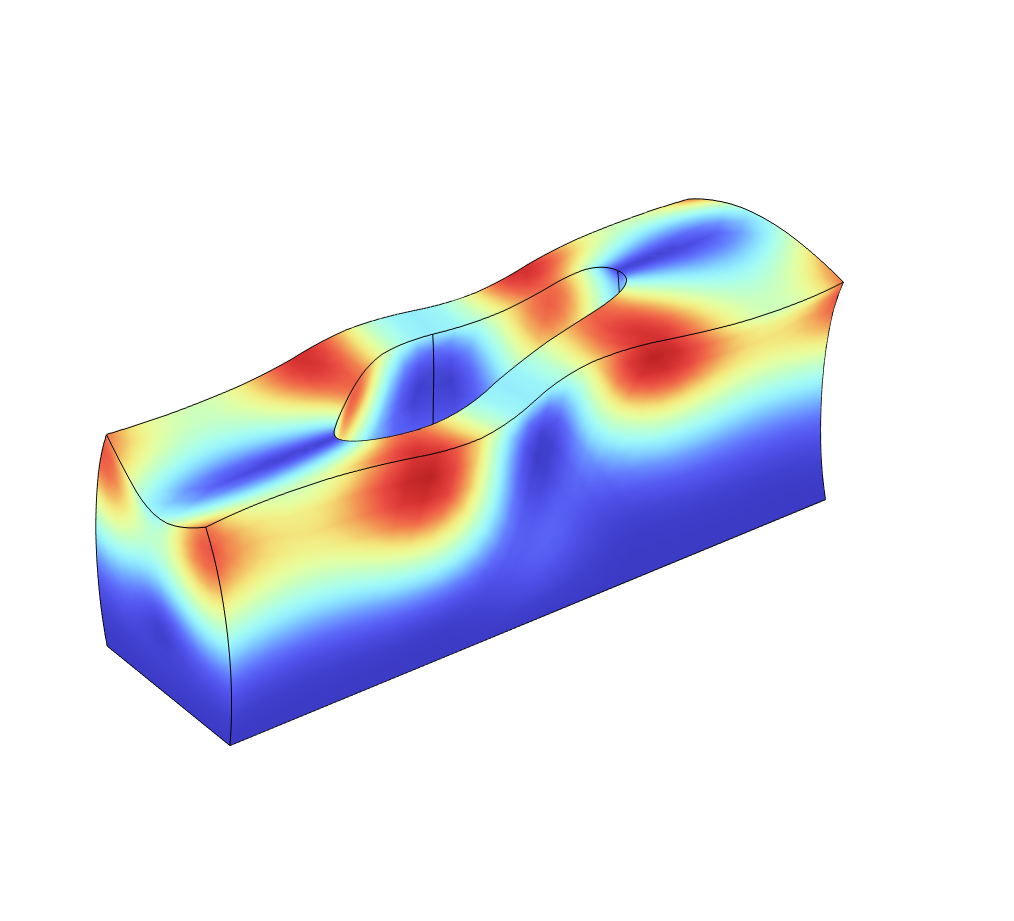
\includegraphics[width=\textwidth]{chapters/theory/modeshape_7.png}
		\end{center}
		\subcaption{}%
		\label{fig:ms7}
	\end{subfigure}
	\begin{subfigure}[]{0.24\textwidth}
		\begin{center}
			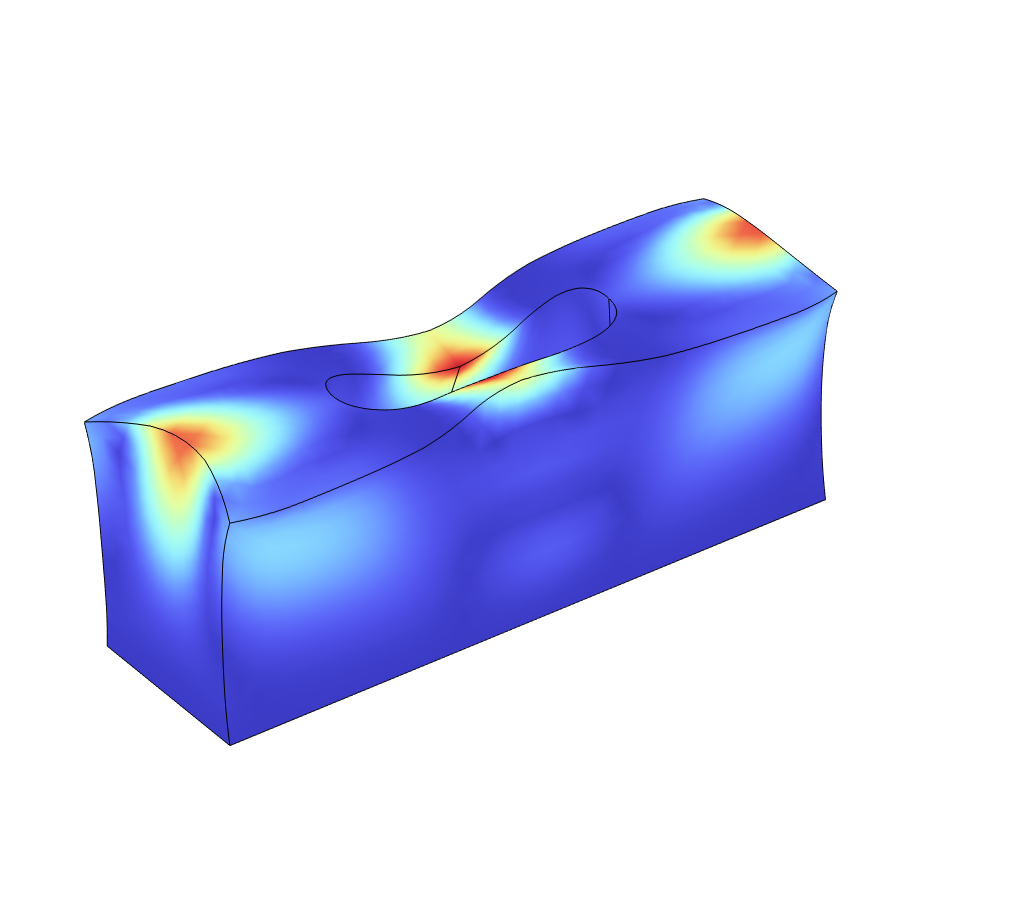
\includegraphics[width=\textwidth]{chapters/theory/modeshape_8.png}
		\end{center}
		\subcaption{}%
		\label{fig:ms8}
	\end{subfigure}

	\caption{%
		Mode shapes for the lowest eight modes at $k=0.9 \pi / a$.
		The color denotes the absolute value of the displacement,
		and the scale is normalized for each figure.
	}%
	\label{fig:modeshapes}
\end{figure}
\tododec{At some point write about phonons? I haven't really had to care about
the fact that excitations are discrete so if I talk about it it'd just for applications...}

\chapter{Inverse Design}

Inverse design is a design paradigm where the design of a device is guided fully by
the desired characteristics.
These desired characteristics are quantified through what is called an objective
function%
\footnote{Also called \emph{figure of merit (FoM)}.}%
, which I will denote $\fobj$,
that should be maximized.
When coupled with \emph{adjoint simulation}, which is a clever way to compute
gradients, and gradient based optimization
algorithms, this is a very powerful methodology.

An overview of the design process is as follows:
\begin{enumerate}
	\item Initialize a random device design.
	\item\label{it:grad} Calculate the gradient of the design through the adjoint method.
	\item Update the device design using the gradient according to the optimization algorithm.
	\item If the device performance is good enough, terminate optimization, else
		return to step~\ref{it:grad}.
\end{enumerate}

\section{Adjoint Simulation}

Adjoint simulation is a way to compute the gradient of $\fobj$ with respect to
the design, which in our case means with respect to the material parameters.
I will in this section first give a general derivation, following
reference~\cite{giles_introduction_2000}.
In \cref{sec:spec_der} I will then derive the specifics when applying this to
acoustics.

\subsection{General Derivation}\label{sec:general_derivation}

Let $\fobj$ be a function which depends on some high-dimensional vector $v$.
The vector $v$ can be calculated by solving the linear equation
$A v = b$, where $b$ is a fixed vector and $A$ is a matrix that depends on a
vector of design parameters $p$.
This could be the acoustics equation, but it might also be the analogous
equation for photonics, or something completely different like fluid dynamics.
I will refer to the process of solving this equation as a simulation, since for
this thesis it is solved through the simulation software COMSOL.
The overall goal is to find the parameters $p$ that maximize the objective
function $\fobj$.
The goal of adjoint simulation is to find $\diff{\fobj}{p}$.
This can be expanded through the chain rule as
\begin{equation}
	\diff{\fobj}{p} = \diff{\fobj}{v} \diff{v}{p}.
\end{equation}
To find the latter factor we do
\begin{align}
	\diff{}{p} [Av = b] &\implies \diff{A}{p} v + A \diff{v}{p} = 0\\
						&\implies A\diff{v}{p} = -\diff{A}{p}
						v.\label{eq:direct_dvdp_solve}
\end{align}
Thus, if we can find a $\tilde v$ such that
\begin{equation}\label{eq:vtilde}
	\diff{\fobj}{v} = \tilde v A
\end{equation}
then
\begin{align}
	\label{eq:dfdp_vtilde}
	\diff{\fobj}{p} &=
	\tilde v A \diff{v}{p}\\
	&=
	-\tilde v \diff{A}{p} v.
\end{align}
Finding $\tilde v$ from \cref{eq:vtilde} amounts to solving the so called
\emph{adjoint problem}:
\begin{equation}
	A^\dagger \tilde v^\dagger = \diff{\fobj}{v}^\dagger
\end{equation}
hence the name adjoint method.
As it turns out, $A$ is in many cases symmetric (or self-adjoint) which means that this is simply a normal
simulation but with $\difs{\fobj}{v}^\dagger$ as the source.
Thus, to obtain the derivative we just need to run an additional
simulation with a different input.

Now you might be wondering: what have we gained by this?
Let $n$ be the dimension of $v$, $m$ the dimension of $p$ and $l$ the dimension
of $b$.
This means that $A$ is a matrix with dimension $l\times n$ and $\difs{A}{p}$ is
a rank three tensor with dimension $m\times l\times n$.
Thus solving for $\difs{v}{p}$ from equation \cref{eq:direct_dvdp_solve}
means solving for an $n \times m$ matrix, which much more computationally
expensive than solving for just a vector of dimension $n$.

\subsection{Specific derivation with acoustics}\label{sec:spec_der}

Now we turn to the specific case of acoustic devices.
Here $A v = b$ is replaced by the acoustic field equation (\cref{eq:gov_eq}):
\begin{equation}\label{eq:sim_eq}
	\hat A_{ik} u_k = F_i.
\end{equation}
Instead of vectors, like we saw in \cref{sec:general_derivation}, these quantities are now functions%
\footnote{%
	Vector-valued funcitons, but that is not the important part here.
}
of $\vec x$.
Analogously to the vector of design parameters we now have a \emph{design field}
$p(\vec x)$,
and analogously to $\fobj$ being a function of a vector, this $\fobj$ is a
function of a function, i.e.\ a \emph{functional}.
For a quick overview of functionals and their derivatives, see
\cref{box:functionals}.

\begin{mybox}[breakable, parbox=false, label=box:functionals]{On functionals and their derivatives}
	\tododec{
		Big fat box on functionals and their derivatives. I think this should be
		included somewhere, since very few of my peers know what a functional
		derivative is... Not really sure how though. I kinda like the thought of
		putting it in a box like this.
		Alternatively, I could put it in an appendix.
	}
Our $\fobj$ is no longer a function, but rather a \emph{functional}, and thus
we need to use the functional derivative instead of the ordinary derivative.
One can think of a functional as a function of a function,
i.e.\ something that maps an element of a function space to a scalar number.
There are also functionals which depend on both a function and a real number,
or on multiple functions.
Below I will give an overview of the notational conventions I use,
and then give the definition of the functional derivative as well as some useful
properties of it.

Let $\mathcal{Y}$ be a function space of functions $\R \to \R$.
A functional $F:\mathcal{Y} \to \R$ evaluated at the function
$f\in\mathcal{Y}$
is denoted with the function in square brackets: $F[f]$.
Note that in principle, $F$ is the functional while $F[f]$ is just a
number,
analogously to how $f$ is a function while $f(x)$ is a real number.
If the functional additionally depends on a real number,
$G:\mathcal{Y} \times \R \to \R$,
that is put in round brackets: $G[f](x)$.

The functional derivative of $F$ with respect to its function argument
is a functional $\mathcal{Y} \times \R \to \R$ denoted $\difs.f.{F[f]}{f}$.
In this expression, $f$ is technically a dummy function, writing
$\difs.f.{F[g]}{g}$ is exactly the same functional.
However, often the argument of $F$ is omitted and the function in the
denominator is named in accordance with the names in the definition of the
functional.
Furthermore, the same notation is also often used to denote the functional
derivative evaluated at a certain function.
For example, if we define a functional taking two function arguments
$F[f_1, f_2] = \int f_1(x) + f_2(x) \dl x$, one can write
\begin{align}
	\diff.f.{F}{f_2}(x)
	&& \text{meaning}&\quad \diff.f.{F[g_1, g_2]}{g_2}(x)\\
	\diff.f.{F}{f_2}(x)
	&& \text{meaning}&\quad \diff.f.{F[g_1, g_2]}{g_2} [f_1, f_2](x)
\end{align}
where in the latter case, $f_1$ and $f_2$ are specific functions defined
previously.
Also note that the scalar argument to the functional derivative can be put
either in the denominator or after, depending on what is more convenient.
Oftentimes, when the functional being differentiated is a long expression and is
placed after the fraction, the argument is placed in the denominator:
\begin{equation}
	\diff.f.{F}{f}(x) = \diff.f.{F}{f(x)} = \diff.f.*{F}{f(x)}
\end{equation}

The functional derivative is defined by
\begin{equation}
	\int \diff.f.{F}{f} (x) \varphi(x) \dl x
	= \diff*{F[f + \varepsilon \varphi]}{\varepsilon}
\end{equation}
where $F$ is a functional of $f$ and $\varphi$ is an arbitrary test function.
I will use two properties of the functional derivative:
\begin{itemize}
	\item If $F$ is the functional $F[f](y) = f(y)$,
		then $\difs.f.{F(y)}{f}(x) = \delta(y-x)$.
	\item The chain rule: if $F$ is a functional with one function argument,
		$G$ is a functional with one function and one real argument,
		and $H$ is the functional defined as $H[f] = F[G[f](y)]$,
		then
		\begin{equation}
			\diff.f.{H}{f}(x)
			= \int \diff.f.{F}{G[f]}(y) \diff{G(y)}{f}(x) \dl{y}
		\end{equation}
\end{itemize}
\end{mybox}

For simplicity I will limit myself to the case where the objective function is
an overlap integral of the displacement field $u_k(\vec x)$ with some function
$\varphi_k^*(\vec x)$:
\begin{equation}
	\fobj[\vec u] = \int_\Omega u_i(\vec x) \varphi_i^*(\vec x) \dl{\vec x}.
\end{equation}
where $\Omega$ is the domain of $\vec u$.
Such an integral is an inner product in the space of functions on
$\Omega$.

Analogously to the general derivation in \cref{sec:general_derivation},
the chain rule is used to expand
$\difs.f.{\fobj}{p}(\vec x)$, see \cref{box:functionals} for the form of the
chain rule for the functional derivative.
However, because $\vec u$ is in general complex, I will split it into its real and
imaginary components: $\vec u = \vec v + i \vec w$.
\begin{equation}
	\label{eq:chain_rule}
	\diff.f.{f_\text{obj}}{p}(\bm x)
	=
	\int_\Omega \dl{\bm y} 
	\diff.f.{f_\text{obj}}{v_i}(\bm y)
	\diff.f.{v_i(\bm y)}{p}(\bm x)
	+
	\diff.f.{f_\text{obj}}{w_i}(\bm y)
	\diff.f.{w_i(\bm y)}{p}(\bm x)
\end{equation}
The first factor of each of the two terms is easy enough to calculate:
\begin{align}
	\diff.f.{f_\text{obj}}{v_i}(\bm y) &=
	\diff.f.*{
		\int_\Omega u_j(\bm x) \varphi_j^*(\bm x) \dl{\bm x}
	}{v_i(\bm y)}\\
	&= \int_\Omega
	\diff.f.*{
		u_j(\bm x) \varphi_j^*(\bm x)
	}{v_i(\bm y)} \dl{\bm x}\\
	&= \int_\Omega
	\delta(\bm x - \bm y) \delta_{ij} \varphi_j^*(\bm x)
	\dl{\bm x}\\
	&= \varphi_i^*(\bm y)
\end{align}
and
\begin{align}
	\diff.f.{f_\text{obj}}{w_i}(\bm y) &=
	\diff.f.*{
		\int_\Omega u_j(\bm x) \varphi_j^*(\bm x) \dl{\bm x}
	}{w_i(\bm y)}\\
	&= \int_\Omega
	\diff.f.*{
		u_j(\bm x) \varphi_j^*(\bm x)
	}{w_i(\bm y)} \dl{\bm x}\\
	&= \int_\Omega
	i \delta(\bm x - \bm y) \delta_{ij} \varphi_j^*(\bm x)
	\dl{\bm x}\\
	&= i \varphi_i^*(\bm y)
\end{align}
which gives us
\begin{align}
	\diff.f.{f_\text{obj}}{p}(\bm x)
	&=
	\int_\Omega \dl{\bm y}
	\varphi_i^*(\bm{y})
	\diff.f.{v_i(\bm y)}{p}(\bm x)
	+
	i \varphi_i^*(\bm{y})
	\diff.f.{w_i(\bm y)}{p}(\bm x)\\
	&=
	\int_\Omega \dl{\bm y}
	\varphi_i^*(\bm{y})
	\Re\left(\diff.f.{u_i(\bm y)}{p}(\bm x)\right)
	+
	i \varphi_i^*(\bm{y})
	\Im\left(\diff.f.{u_i(\bm y)}{p}(\bm x)\right)\\
	&=
	\int_\Omega \dl{\bm y}
	\varphi_i^*(\bm{y})
	\diff.f.{u_i(\bm y)}{p}(\bm x)
	\label{eq:dfdp_as_dudp_integral}
\end{align}
To find $\difs.f.{u_i(\bm y)}{p}(\bm x)$ we apply $\difs.f.{}{p(\bm x)}$ to
\cref{eq:sim_eq}, which gives us
\begin{equation}\label{eq:dAdpu_Adudp}
	0 =
	\diff.f.{\hat A_{ik}}{p}(\vec x) u_k(\bm y)
	+
	\hat A_{ik} \diff.f.{u_k(\bm y)}{p}(\bm x)
\end{equation}

% The point of inverse design is that we now want to find an adjoint field
% $\tilde u_i(\bm y)$
% such that the integral in \cref{eq:dfdp_as_dudp_integral} is
Just like \cref{eq:dfdp_vtilde},
we want an adjoint field $\tilde{\vec u}$
such that the integral in \cref{eq:dfdp_as_dudp_integral} is
\begin{equation}\label{eq:phi_dudp_integral}
	\int_\Omega \dl{\bm y}\,
	\varphi_i^*(\bm y)
	\diff.f.{u_i(\bm y)}{p}(\bm x)
	=
	\int_\Omega \dl{\bm y}\,
	\tilde u_i(\bm y)
	\hat A_{ik}
	\diff.f.{u_k(\bm y)}{p}(\bm x)
\end{equation}
which by \cref{eq:dAdpu_Adudp} is equal to
\begin{equation}\label{eq:an_integral}
	-\int_\Omega \dl{\bm y}\,
	\tilde u_i(\bm y)
	\diff.f.{\hat A_{ik}}{p}(\vec x)
	u_k(\bm y).
\end{equation}
The adjoint field is found by solving the adjoint problem:
\begin{equation}
	\hat A_{ik}^\dagger \tilde{u}_k = \varphi^*_i,
\end{equation}
where the adjoint operator $\hat A_{ik}^\dagger$ is defined through
\begin{equation}
	\int_\Omega f(\vec x) \left(\hat A_{ik} g(\vec x)\right) \dl{\vec x}
	=
	\int_\Omega \left(\hat A_{ik}^\dagger f(\vec x)\right) g(\vec x) \dl{\vec x}.
\end{equation}
To further simplify this expression, the dependence of $\hat A$ on $p$ must be
specified.
A linear dependence is proposed here, though extending the formula to more
complicated dependences is rather easy.
Taking $\rho(\vec y) = \rho^0 p(\vec y)$
and $C_{ijkl}(\vec y) = C_{ijkl}^0 p(\vec y)$
in the definition of $\hat A_{ik}$ from \cref{eq:A_def}
implies 
\begin{align}
	\diff.f.{\hat A_{ik}(\vec y)}{p}(\vec x)
	= -\rho^0 \omega^2 \delta_{ik} \delta(\vec x - \vec y)
	- \partial_j\left(C_{ijkl}^0\delta(\vec x - \vec y) \partial_l \placeholder\right)\\
	= -\rho^0 \omega^2 \delta_{ik} \delta(\vec x - \vec y)
	- 2 C_{ijkl}^0\delta(\vec x - \vec y)\partial_j \partial_l.
\end{align}
Plugging this back into the integral in \cref{eq:an_integral} gives
\begin{equation}
	\omega^2 \rho^0 \tilde u_i(\vec x) u_i(\vec x)
	+ 2 C_{ijkl}^0 \tilde u_i(\vec x) \partial_j \partial_l u_k(\vec x)
\end{equation}
which is comparatively easily evaluated.

% \todoblk{The infamous integral. Still am not entirely sure about it, but I
% haven't thought more about it since I abandoned that.}
\tododec{Comment from PB:
	it might be nice to clarify at which point one can see that the adjoint simulation would result in the solution u tilde
	you could consider writing a short summary at the end of the chapter where you explain step by step how inverse design is practically done. E.g.: 
	1. We are solving the system with the regular acoustic field equation for a certain p and receive u
	2. we are interested in df/dp so that we know how to change p in order to maximize f
	3. df/dp was calculated in eqn X. 
	I think this would be instructive for the reader :)
}

\section{Optimization Algorithms}

\todowrt{rephrase first sentence}
In the last section I painstakingly derived how one can obtain the gradient,
and in this section I will attempt to justify that by describing how one can use
the gradient.
I will begin by describing the advantages of gradient based optimization
algorithms over those that don't use the gradient.
Following that I describe the algorithm that I used, as well as some of it's
predecessors.

An optimization algorithm is an algorithm for finding the optimum of a function.
The function is often called the \emph{objective function} or the \emph{cost
function}.
A very naive optimization method would be to simply try some number of inputs
and then choose the one with the highest function value.
This requires a large number of points before a good value is found,
meaning that it takes a long time.
An improvement to this method is to use the information gained from the points
already tried to decide which points to try next.
If some point has a bad value, then try somewhere else; if some point has a good
value, try another close by.
Examples of algorithms that do this are bayesian optimization, particle swarm
optimization, and various forms of genetic
algorithms~\cite{schneider2019benchmarking}.
However, if the domain of the objective function is very high-dimensional,
``close by'' is a very large space.
For such functions, it is essential to know in which direction the
function increases.
That is why gradient based optimization algorithms are so powerful;
they enable us to quickly find the right direction to go in for best
improvement.

% \tododec{%
% 	Curiosity that could be included:
% 	If you have a linear function (which all functions are if you zoom in far
% 	enough) $f(x) = v\cdot x + k$, and take a random step (random meaning random
% 	step in $[-\epsilon, \epsilon]$ in each dimension)
% 	then the expected improvement (given that you don't go downhill, in which
% 	case you can just stay where you are).
% 	% Curiosity that could be included. If you have a linear function
% 	% $f(x) = v\cdot x + k$, what is the probability that you will significantly
% 	% (say more than 10\% of optimal step) increase $f$ with a random unit
% 	% length step?
% 	% Optimal: step in $\hat v$, $\Delta f = v\cdot \hat v = \norm{v}$.
% 	% Probability of 10\% of this: $\int_{0.1}^1 (1-x^2)^{n/2} \dl x / \int_{-1}^1
% 	% \cdots$
% 	% use $(1-x^2)^n \approx \exp(-n x^2)$.
% 	% Approaches 0 very very quickly, at 10000 dimensions it's like \num{1e-45} or something.
% 	% Or maybe give the expected improvement given that you take the max of
% 	% current result and next result.
% }

\subsection{Gradient Descent}

The simplest gradient based optimization algorithm is called \emph{gradient
descent}.
Like all of the algorithms I will describe it is an iterative algorithm,
meaning that it generates a sequence of points that converges to an optimum,
and the next point in the sequence is derived from the previous ones.
In the case of gradient descent, the next point is gotten by
\begin{equation}
	p_n = p_{n-1} + \eta g_{n-1}
\end{equation}
where $\eta$ is the so called \emph{learning rate} and $g_{n-1}$ is the gradient
of the objective function at $p_{n-1}$.
For ordinary gradient descent the learning rate would be fixed,
and choosing an appropriate value for this parameter is one of the problems of
this method.
If a too high value is chosen, then the steps taken will be too large and the
optimium might be missed entirely.
A too low value results in too small steps which will yield a slow convergence.
Almost all gradient descent implementations use a so called learning schedule,
which means that $\eta$ is not constant during the optimization.
This introduces the additional problem of how to choose how fast and between
which values it should change.

\subsection{Adaptive Moment Estimation (ADAM)}

The \gls{adam} algorithm is an improved version of gradient descent.
It has three main differences:
\begin{enumerate}
	\item Each dimension has a separate learning rate.
	\item The learning rate is automatically set from the previously seen gradients.
	\item The evolution carries some momentum.
\end{enumerate}
\Cref{fig:adam_vs_gd} shows the difference in performance between \gls{adam}
and \gls{gd}.
With a slightly too large learning rate, the \gls{gd} algorithm gets stuck in an
oscillation and makes very little progress towards the minimum.
If the learning rate is decreased, the oscillations disappear but the stepsize
is now too small to make it all the way to the true minimum. 
Since the \gls{adam} algorithm has some momentum, the motion along the valley
gets compounded while the motion perpendicular gets dampened which means that
the oscillations are not as much of a problem.
The adaptive learning rate also means that the algorithm doesn't get stuck
prematurely due to the small gradient at the bottom of the valley.
Admittedly, this objective function is specifically chosen to showcase the
advantages of \gls{adam}, but it has been shown to outperform \gls{gd} in almost
all cases~\cite{kingma2017adam}.
\begin{figure}[htpb]
	\centering
	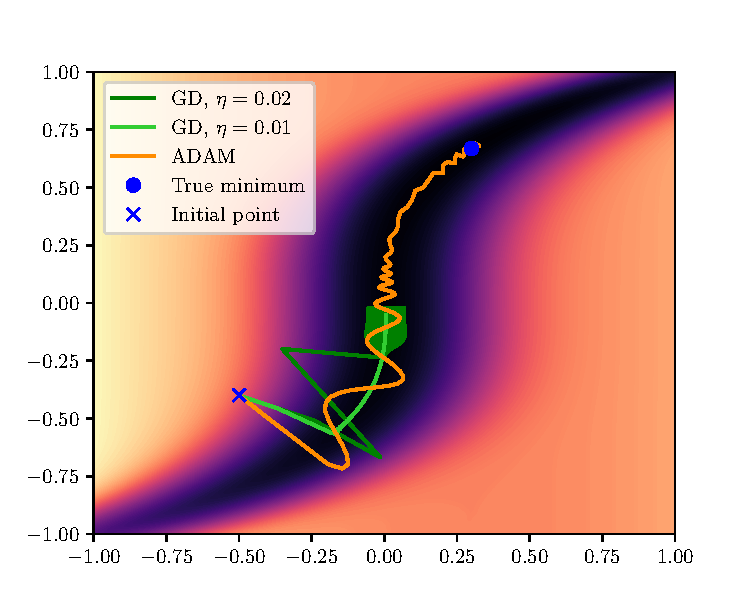
\includegraphics{chapters/theory/adam_vs_gd_plot.pdf}
	\caption{
		A comparison between \gls{adam} and \gls{gd} in an optimization
		landscape with a narrow canyon. The two different \gls{gd} algorithms
		are shown with 1000 steps, while 200 steps with the \gls{adam} algorithm
		are shown.
	}
	\label{fig:adam_vs_gd}
\end{figure}

\begin{listing}
	\begin{minted}{Python}
def adam(theta_0, get_gradient, alpha,
		beta_1, beta_2, epsilon, n_iter):

	m = np.zeros(theta_0.shape)
	v = np.zeros(theta_0.shape)
	theta = theta_0

	for i in range(n_iter):
		g = get_gradient(theta)
		# Update biased first moment estimate
		m = beta_1 * m + (1-beta_1) * g
		# Update biased second moment estimate
		v = beta_2 * v + (1-beta_2) * g**2

		# Compute the bias-corrected estimates
		m_hat = m / (1 + beta_1**i)
		v_hat = v / (1 + beta_2**i)

		# Update theta
		theta -= alpha * m_hat / (np.sqrt(v_hat) + epsilon)
	\end{minted}
	\caption{%
		Pseudocode for the ADAM algorithm. See \cite{kingma2017adam} for a more
		in depth discussion of the algorithm.
	}
	\label{lst:adam}
\end{listing}
